\section{Banc de couloir : effet séparé des paramètres du sol mouillé}
\label{sec:annexe-couloir}

Avant les campagnes sur la piscine, un banc de couloir sépare les trois paramètres par
lesquels le sol mouillé agit : la vitesse souhaitée $s$, le temps de relaxation $\tau$ et
l'accélération maximale $a_{\max}$ de la bande mouillée ($4\leq x<\SI{8}{\metre}$). On part
d'une référence où le mouillé est identique au sec ($\tau=\SI{0.3}{\second}$,
$a_{\max}=\SI{3}{\metre\per\second\squared}$, $s=\SI{1.5}{\metre\per\second}$), puis on
reprend un seul paramètre du mouillé à la fois ($\tau=\SI{0.6}{\second}$,
$a_{\max}=\SI{0.7}{\metre\per\second\squared}$, $s=\SI{1}{\metre\per\second}$), et enfin des
combinaisons. Les 24 agents, leurs placements et les cinq graines sont les mêmes pour toutes
les variantes, et les écarts au passage médian sont appariés graine par graine. Ces valeurs
sont illustratives : il s'agit de séparer des mécanismes, pas de calibrer la piscine. Une
mesure incomplète est refusée, sans exclure en silence un agent ou une graine.

\begin{table}[ht]
\centering
\caption{Sol mouillé, un paramètre à la fois. Moyennes sur cinq graines ; l'écart-type, de
l'ordre de \SI{0.003}{\second} sur les temps, est omis. Freinage : distance parcourue dans la
bande avant de revenir à \SI{5}{\centi\metre\per\second} de la vitesse souhaitée. Contacts :
durée cumulée des paires à moins de \SI{1}{\milli\metre} du contact dans la bande.}
\label{tab:mouille}
\begin{tabular}{lrrrr}
\toprule
Variante & $t_{50}$ (s) & Traversée (s) & Freinage (m) & Contacts (paires$\cdot$s) \\
\midrule
Référence (mouillé = sec) & 7,082 & 2,672 & 0,01 & 0 \\
Relaxation seule & 7,083 & 2,677 & 0,01 & 0 \\
Adhérence seule & 7,082 & 2,672 & 0,01 & 0 \\
Vitesse seule & 8,368 & 3,860 & 0,53 & 65 \\
Vitesse + adhérence & 8,324 & 3,816 & 0,73 & 63 \\
Complet & 8,223 & 3,716 & 1,86 & 55 \\
\bottomrule
\end{tabular}
\end{table}

\begin{figure}[ht]
\centering
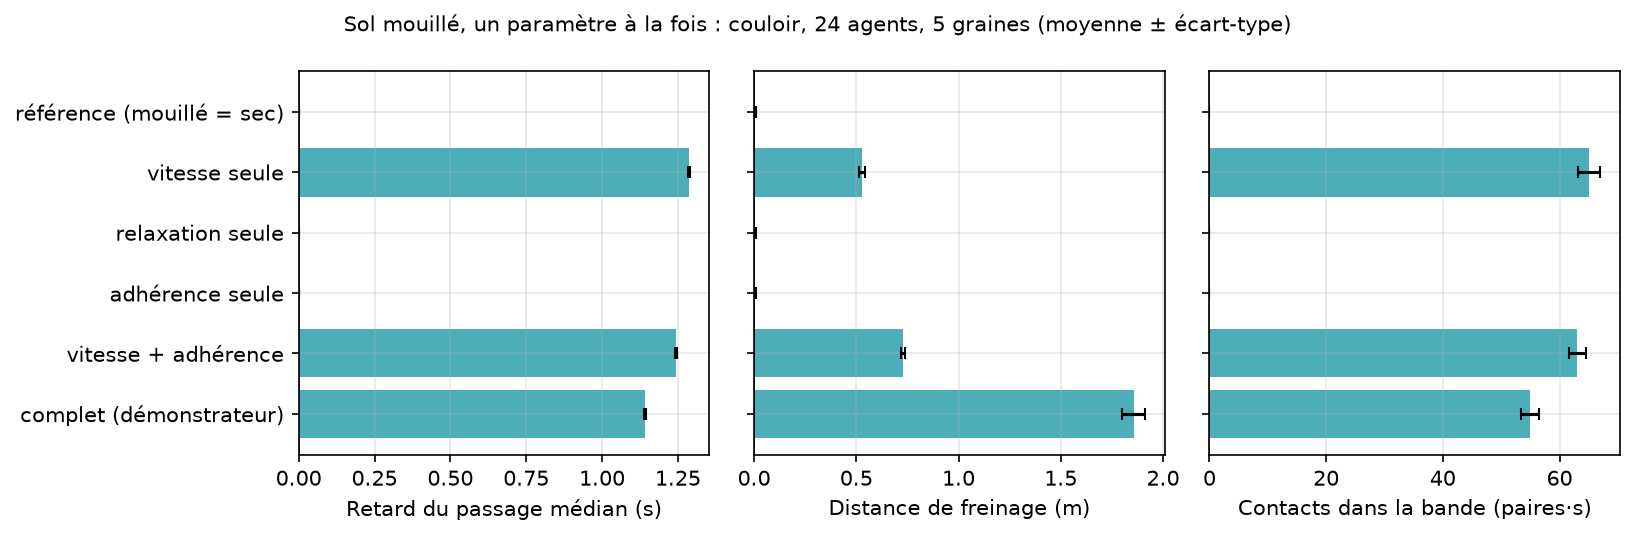
\includegraphics[width=\linewidth]{fig07_mouille_un_parametre}
\caption{Retard du passage médian par rapport à la référence, distance de freinage et
compression dans la bande mouillée, pour chaque variante. Reproduction :
\texttt{viscocrowd comparer-mouille experiments/couloir.yaml --figure report/figures}
(manifeste, \texttt{fig07}).}
\label{fig:mouille}
\end{figure}

À vitesse souhaitée identique, prendre seulement le $\tau$ ou seulement le $a_{\max}$ du
mouillé ne change rien : le passage médian bouge de moins de \SI{1}{\milli\second} et aucun
contact n'apparaît (tableau~\ref{tab:mouille}, figure~\ref{fig:mouille}). Dans ce couloir
droit, les agents arrivent déjà à leur vitesse souhaitée, et rien ne leur demande d'accélérer,
de freiner ou de tourner. L'inertie ne peut agir que lors d'un changement de vitesse
souhaitée, d'un virage, d'un contournement ou d'une collision.

Seule, la vitesse plus faible du mouillé retarde le passage médian de \SI{1.29}{\second}. Les
agents de tête ralentissent avant ceux qui les suivent : la file se comprime à l'entrée de la
bande, et 65~paires$\cdot$s de contacts apparaissent, contre aucun dans la référence.

Avec une adhérence faible, le freinage demandé, $(1{,}5-1)/0{,}3\approx\SI{1.7}{\metre\per\second\squared}$,
dépasse $a_{\max}=\SI{0.7}{\metre\per\second\squared}$ et se trouve borné. La distance de
freinage passe de 0,53 à \SI{0.73}{\metre}, puis à \SI{1.86}{\metre} quand la relaxation du
mouillé s'ajoute. Les agents ralentissent plus progressivement, et la compression diminue (63
puis 55~paires$\cdot$s). Dans ce couloir sans virage ni goulot, l'inertie étale donc le
ralentissement au lieu de provoquer des chocs. C'est devant une porte, où il faut s'arrêter et
repartir, qu'elle peut coûter du débit (section~\ref{sec:e4}).
